\chapter{Force électrique et loi de Coulomb}
Les particules possédant une charge de même signe se repoussent et celles possédant une charge de signe contraire s'attirent. Il existe donc une force s'exerçant entre-elles.
C'est à partir des travaux de Charles Coulomb (1736 - 1806) que s'élabore progressivement la loi permettant de calculer les caractéristiques de celle-ci.
\begin{encadre}
    \motcle{Loi de Coulomb} : \(F=k_0 \frac{q_1 \cdot q_2}{r^2}\)
    où:
    \begin{itemize}[label=\textbullet]
        \item \(F\) est l'intensité de la force, en \([N]\),
        \item \(k_0\) est la constante de Coulomb, \(k=9 \times 10^{9} [N \cdot m^2 \cdot C^{-2}]\) dans le vide,
        \item \(q_1\) et \(q_2\) sont la valeur de la première et de la deuxième charge, en \([C]\),
        \item \(r\) est la distance entre \(q_1\) et \(q_2\), en \([m]\).
    \end{itemize}
\end{encadre}
On notera la frappante similitude entre la loi de Coulomb et celle de la gravité de Newton, ces deux phénomènes n'ayant pourtant rien en commun.
La constante de Coulomb est généralement écrite sous une autre forme, car elle est une \enquote{conséquence} de constantes plus fondamentales.
\begin{encadre}
    \(k_0=\frac{1}{4 \pi \varepsilon_0}\) où \(\varepsilon_0=8,85 \times 10^{-12} [C^2 \cdot N^{-1} \cdot m^{-2}]\)
    \(\varepsilon_0\) est la permittivité diélectrique du vide. La valeur de \(k\) est pratiquement inchangé dans l'air.
\end{encadre}

\newpage

\section{Exercices}
\begin{exercise}
    Combien d'électrons y'a-t-il dans une charge de \(-1 \mu C\)?
\end{exercise}
\begin{solution}
    \(nb_elec=6,25 \times 10^12\)
\end{solution}

\begin{exercise}
    Calcule la force d'attraction électrique qui s'exerce entre le noyau d'un atome de fer (q=26e) et l'électron qui en est le plus rapproché, sachant que la distance qui les sépare vaut \(1,0 \times 10^{-12}[m]\). On considère chaque charge comme étant ponctuelle.
\end{exercise}
\begin{solution}
    \(F_{elec}=5,98 \times 10^{-3}[N]\)
\end{solution}

\begin{exercise}
    À quelle distance faut-il placer deux charges de respectivement 0,01[C] et -0,005[C] pour que s'exerce entre-elles une force de 0,4[mN]?
\end{exercise}
\begin{solution}
    \(r=3,35 \times 10^4 [m]\)
\end{solution}

\begin{exercise}
    Jusqu'à quel point faut-il approcher deux électrons pour que la force qui s'exerce entre-eux soit égale au poids de l'un deux sur Terre?
    Pour rappel : \(G=6,67 \times 10^{-11}\) et \(m_e=9 \times 10^{-31} [kg]\)
\end{exercise}
\begin{solution}
    \(r=5,108[m]\)
\end{solution}


\begin{exercise}
    Compare la force s'exerçant entre deux charges de 1[C] situées à 10[cm] de distance à la force de gravité s'exerçant entre elles si elles sont portées par des masse sphérique de \(1 [kg]\) chacune.
    \begin{enumerate}[label=\textbullet]
        \item \(G=6,67 \times 10^{-11}\)
        \item \(r_{Terre-Lune}=380000[km]\)
    \end{enumerate}
\end{exercise}
\begin{solution}
    La force électrique est \(10^20\) fois plus grande. Lorsqu'on compare la force électrique à la force gravifique entre deux corps, la force gravifique est généralement négligeable.
\end{solution}

\begin{figure}[h!]
    \centering
    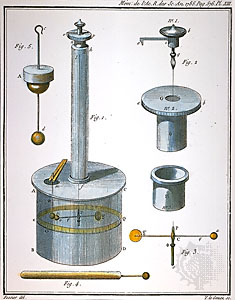
\includegraphics[width=0.6\linewidth]{balance_coulomb.jpg}
    \caption{La balance à torsion de Coulomb, l'instrument utilisé pour réaliser ses observations.}
    \label{balance_coulomb}
\end{figure}
